\documentclass{article}
\usepackage{ucs}
\usepackage[utf8x]{inputenc}
\usepackage{graphicx}
\title{GreenFlow: Reducering af brændstofforbrug ved hastighedstilpasning til trafiklys}
\date{}
\begin{document}
\maketitle

\noindent Ved kendskab til trafiksignalerne kan den enkelte bil tilpasse sin hastighed således det næste kryds nåes i det øjeblik det skifter til grønt.
I mange tilfælde kan standsninger helt undgåes hvorved man opnår et jævnt flow gennem trafiklysene.
Herved reduceres den dyre acceleration.
Simuleringer viser at brændstofforbruget kan mindskes med ca. 25 \% for den enkelte bilist uden nævneværdig negativ påvirkning af øvrig trafik.

\noindent
Besparelsen opnås allerede for den første bil, der bruger GreenFlow og bibeholdes som flere biler begynder at benytte systemet. 
Der er en minimal investering for den enkelte bilist som dirkte får glæde af brændstofbesparelserne.

%\noindent Systemet fungerer bedst uden for myldretiden og med tidsstyret lyskryds, men kan også %bruges i andre tilfælde, dog med et potentielt mindre udbytte for bilisterne.

\noindent GreenFlow implementeres på en smartphone, der udregner og viser hvilken hastighed bilisten skal køre for at nå det næste grønne lys.
For at systemet kan fungere optimalt, kræver det adgang til aflæsning af trafiksignalernes tilstand og at bilisten angiver den rute han vil følge.
GreenFlow har derfor få invisteringsudgifter men høj udbytte for bilisterne.

\vspace{15mm}
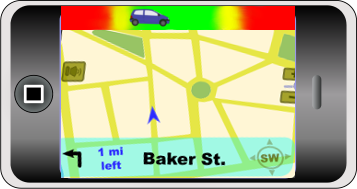
\includegraphics[width=1\textwidth]{images/product.png}
\end{document}













